\section{Aufbau}
\label{sec:Aufbau}
In \autoref{fig:aufbau} ist der verwendete Versuchaufbau zu finden. Er besteht aus einer optischen Schiene, einem
grünen Justierlaser, einem HeNe-Laserrohr mit eingebauten Brewsterfenstern und zwei hochreflektierenden Spiegeln,
die als optischer Resonator dienen. Die Befestigungen der Spiegel können verschoben werden und die Spiegel können
durch planare oder konkave Spiegel aus gewechselt werden. Die Schiene ist $\SI{2,50}{\meter}$ lang und die konkaven
Spiegel haben einen Krümmungsradius von $r=\SI{1400}{\milli\meter}$. Für die Messung stehen noch ein um $2\pi$
drehbarer Polarisationsfilter, ein Wolframdraht, vier optische Gitter, ein Oszilloskop, zwei Photodioden und ein
Schirm zur Verfügung. Diese Bauteile können alle nach Bedarf auf der Schiene angebracht werden.
\begin{figure}
    \centering
    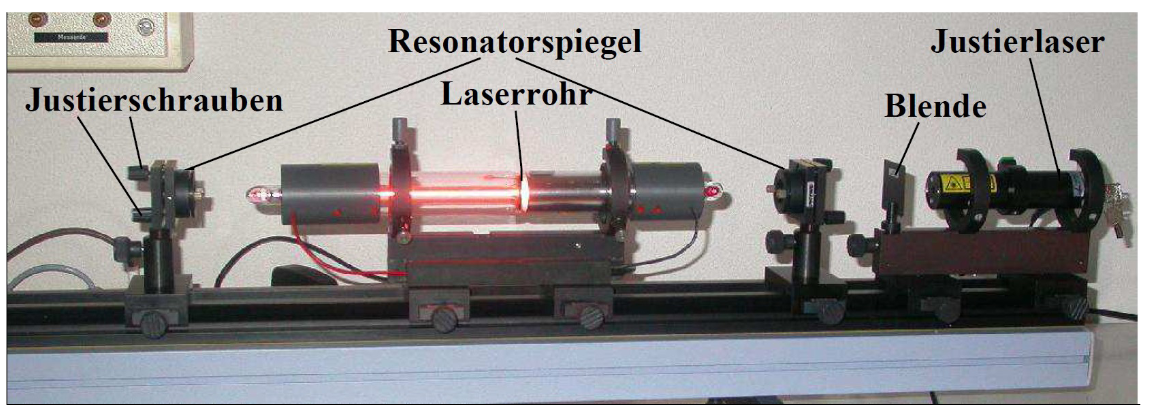
\includegraphics[height=6cm]{content/pics/aufbau.png}
    \caption{Foto des Versuchaufbaus.}
    \label{fig:aufbau}
\end{figure}

\section{Durchführung}
\label{sec:Durchführung}
